\chapter{General approach} \label{chp:general-approach}
	System will be deployed on \gls{AWS} using multiple application and other necessary components to provide stability of the platform. Developed solution will be using \gls{gitlabce}, because in terms of the requirements there is no need to use different more flexible and complex version. 
	\begin{figure}[!htbp]
		\centering
		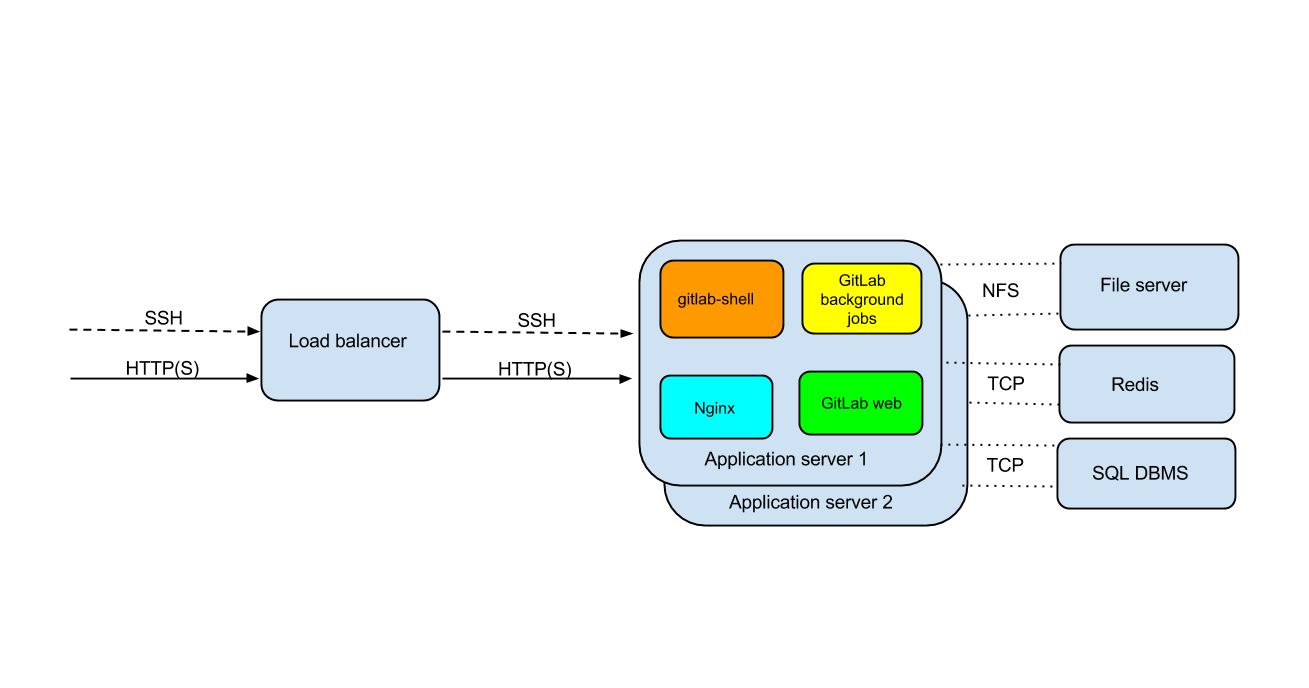
\includegraphics[width=1\textwidth]{img/Config_LB_appservers}
		\caption{Multiple application servers solution for \gls{gitlab} \cite{bib:gitlab-ha}.}
		\label{fig:multiple-application-servers}
	\end{figure} 
	\gls{gitlab} provides set of features for high availability described in details on their web-sides \cite{bib:gitlab-ha}. One of those features shows how to set up this platform for multiple application servers is shown in Figure \ref{fig:multiple-application-servers}.
	Both of the presented platforms connects to three storing/caching components:
	\begin{itemize}
		\item File server -- repository for \gls{git} files;
		\item \gls{redis} -- cache system;
		\item \gls{SQLDBMS} -- database and management system (projects, groups, permission) of platform.
	\end{itemize}
	In further considerations more advanced and redundancy--oriented structure of the components from Figure \ref{fig:multiple-application-servers} will be described. 
	\section{Detailed design} \label{s:general-approach:detailed-design}
	%\section{Implemenetation} \label{s:general-approach:implementation}